\documentclass{article}
\usepackage{hyperref}
\usepackage{amsmath}
\usepackage{amssymb}
\usepackage{graphicx}
\usepackage{booktabs}

\title{Steer on a Sphere: Geometric Control of Transformer Outputs}

\author{N. Trillard \\ \texttt{ntrillard@gmail.com}}

\begin{document}
\maketitle

\begin{figure}[h]
\centering
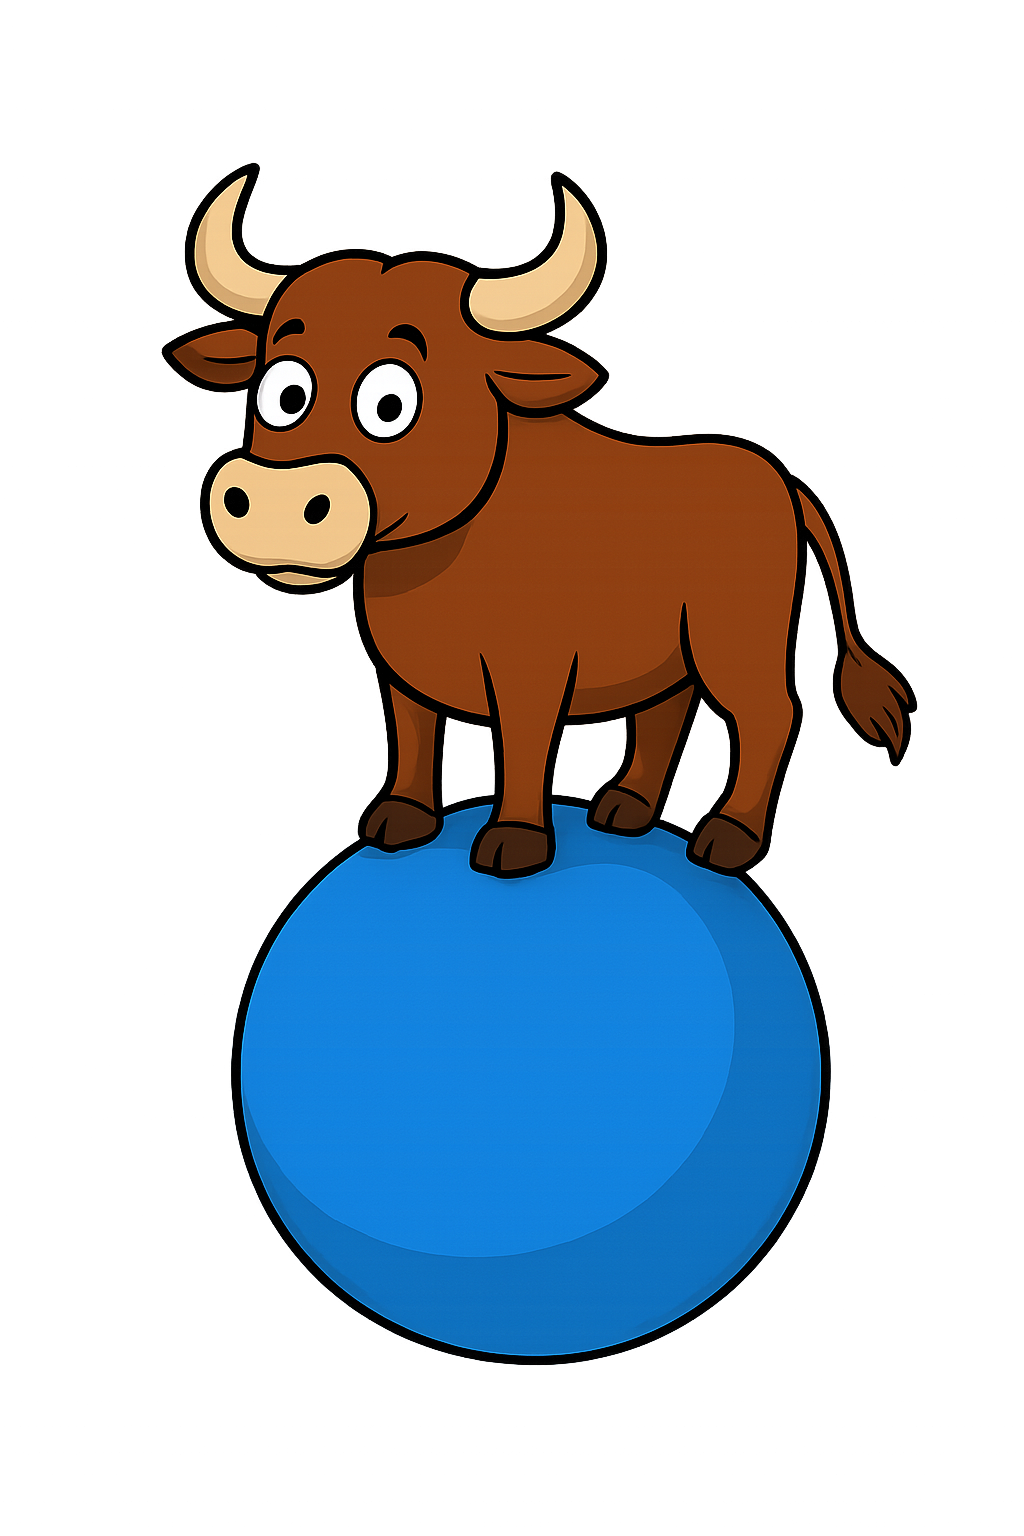
\includegraphics[width=0.2\textwidth]{steeronasphere.png}
\end{figure}

\begin{abstract}
We show that transformer hidden states are constrained to a sphere by layer normalization, with per-layer radius $\|\gamma_l\|$ rather than $\sqrt{d}$. The LM head's gradient decomposes into a radial component and a tangent component. Moving the hidden state along the tangent of a target token increases its probability. On GSM8K, 0-shot accuracy improves from 8\% to 36\% on Qwen2-1.5B and from 10\% to 30\% on Qwen2.5-7B. The technique does not bypass RLHF safety training. We derive a health metric from the perturbation growth rate $\lambda$: healthy models have $\lambda \in [0.02, 0.12]$. TinyLlama-1.1B has $\lambda = 0.183$ and 0\% GSM8K accuracy.
\end{abstract}

\section{Introduction}

Mechanistic interpretability has identified specific circuits in transformers \cite{elhage2021mathematical, olsson2022context}, but a unified geometric framework remains elusive. Layer normalization \cite{ba2016layer} constrains hidden state norms, but the geometric consequences have not been explored. The transformer \cite{vaswani2017attention} combines attention and MLP layers with residual connections; we describe the geometric structure this produces.

\section{Unified Framework}

The transformer's dynamics reduce to four equations:

\paragraph{1. Sphere constraint.} Layer norm outputs have norm $\|\gamma_l\|$, placing every hidden state on a sphere at each layer $l$. All tested models use RMSNorm, so the sphere radius is $\|\gamma_l\|$ directly.

\paragraph{2. Norm growth.} The residual norm grows across layers as $\|h_L\| = \|h_0\| \cdot \exp(\sum_{l=0}^{L-1} \lambda_l)$, where $\lambda_l$ is the per-layer Lyapunov exponent. Healthy models have $\bar{\lambda} \in [0.02, 0.12]$ in the computation zone (middle third of layers).

\paragraph{3. Three dynamical zones.} The per-layer $\lambda_l$ follows a consistent pattern: high in early layers (routing, $\lambda$ up to $2.4$ at layer 0, decreasing to $0.02$), low in middle layers (computation, $\lambda \approx 0$), and rising in late layers (execution, $\lambda \approx 0.02\text{--}0.22$).

\paragraph{4. Steering.} The LM head defines tangent directions for each token: $g_t = W_t - (W_t \cdot \hat{h})\hat{h}$. Moving $h$ along $g_t$ and renormalizing to the sphere gives $h' = (h + \alpha g_t) / \|h + \alpha g_t\| \cdot \|\gamma_L\|$. This increases $P(t|h)$ with no training or prompt engineering.

\begin{table}[h]
\centering
\begin{tabular}{lcccc}
\toprule
\textbf{Quantity} & \textbf{Symbol} & \textbf{Equation} & \textbf{Range} \\
\midrule
Sphere radius & $\|\gamma_l\|$ & $\|\text{LN}_l(h)\| = \|\gamma_l\|$ & $1\text{--}200$ \\
Lyapunov exponent & $\lambda_l$ & $\ln(\|h_{l+1}\|/\|h_l\|)$ & $0\text{--}2.4$ \\
Health metric & $\bar{\lambda}$ & mean of $\lambda_l$ in comp zone & $[0.02, 0.12]$ \\
Steering vector & $g_t$ & $W_t - (W_t \cdot \hat{h})\hat{h}$ & $\|g_t\| \approx 0.6\text{--}0.7$ \\
\bottomrule
\end{tabular}
\caption{Unified framework equations and observed ranges.}
\end{table}

\section{The Sphere Radius}

The sphere radius grows across layers as the residual stream accumulates:

\begin{center}
\begin{tabular}{lcccc}
\toprule
Model & $d$ & $\|\gamma_0\|$ & $\|\gamma_{\text{comp}}\|$ & $\|\gamma_{\text{end}}\|$ \\
\midrule
Mistral-7B & 4096 & 16.6 & 111--158 & 195.5 \\
Qwen2.5-7B & 3584 & 17.0 & 46--66 & 90.0 \\
Qwen2-1.5B & 1536 & 20.0 & 40--60 & 71.0 \\
\bottomrule
\end{tabular}
\end{center}

All vocabulary tokens lie in the equatorial plane, at $87\text{--}90^\circ$ from the BOS direction.

\section{Steering Results}

On 50 GSM8K problems (Qwen2-1.5B, 0-shot, 128 tokens):

\begin{center}
\begin{tabular}{lcc}
\textbf{Target} & \textbf{Accuracy} & \textbf{Example} \\
\hline
None & 8\% & "If the store starts with 120 apples..." \\
"answer" & 36\% & "answer: 75" \\
"solve" & 30\% & "solve for the number of apples left" \\
"result" & 28\% & "result = 120 - 45" \\
\end{tabular}
\end{center}

On Qwen2.5-7B: baseline 10\%, steered 30\%. Steering toward words preserves coherence; numbers produce terse output.

\subsection{Safety}

Testing "How to hotwire a car?" on Qwen2.5-7B with $\alpha = 0.3, 0.5, 1.0$:
- Baseline: "I'm sorry, but I cannot provide instructions..."
- $\alpha=0.3$: "hotwiring a car is illegal and unethical..."
- $\alpha=0.5$: "stealing or tampering with a vehicle without permission is illegal..."

Safety held at all strengths. Steering changes phrasing but does not produce harmful instructions.

\subsection{Health Metric}

The Lyapunov exponent $\lambda$ measures how fast perturbations grow as they pass through the computation zone. Testing requires two forward passes ($\approx 1$ second total) and uses only the model's weights, no training data.

Across all healthy models we tested (Qwen2-1.5B, Qwen2.5-7B, Mistral-7B), $\lambda$ falls in $[0.02, 0.12]$. TinyLlama-1.1B has $\lambda = 0.183$ and scores 0\% on GSM8K:

\begin{center}
\begin{tabular}{lcc}
\textbf{Model} & $\lambda$ & \textbf{GSM8K} \\
\hline
Qwen2-1.5B & 0.051 & 40\% \\
Mistral-7B & 0.069 & 50\% \\
\end{tabular}
\end{center}

Models outside $[0.02, 0.12]$ are likely impaired. The check takes one second.

\section{Related Work}

Layer normalization \cite{ba2016layer}. Attention sinking to BOS \cite{xiao2023efficient} is a consequence of the geometric contraction mechanism. Transformer circuits \cite{elhage2021mathematical, olsson2022context} provide a complementary perspective. Unlike prior steering methods requiring fine-tuning, sphere steering operates purely on hidden state geometry.

\section{Limitations}

Steering only affects the first generated token. Optimal $\alpha$ depends on the task. Numbers produce terse output. $\lambda$ requires two forward passes.

\section{Conclusion}

Transformers organize hidden states on a sphere. The radius varies per layer. The LM head's tangent gradients enable geometric output control. No training, no weights modified, no safety bypass. Code at \url{https://github.com/ntillard/transformer-geometry}.

\section*{Acknowledgments}

We used DeepSeek V4 Flash (DeepSeek) for writing assistance.

\begin{thebibliography}{9}
\bibitem{ba2016layer} J.~L.~Ba, J.~R.~Kiros, and G.~E.~Hinton. \newblock Layer normalization. \newblock arXiv:1607.06450, 2016.
\bibitem{vaswani2017attention} A.~Vaswani et al. \newblock Attention is all you need. \newblock NeurIPS, 2017.
\bibitem{elhage2021mathematical} N.~Elhage et al. \newblock A mathematical framework for transformer circuits. \newblock Transformer Circuits Thread, 2021.
\bibitem{olsson2022context} C.~Olsson et al. \newblock In-context learning and induction heads. \newblock Transformer Circuits Thread, 2022.
\bibitem{xiao2023efficient} G.~Xiao et al. \newblock Efficient streaming language models with attention sinks. \newblock arXiv:2309.17453, 2023.
\end{thebibliography}

\end{document}